\chapter{Introduction}
The amount of Internet connected devices has for the past few years been rapidly increasing and is still doing so. The latest forecasts
estimates that there will be about 27 billion devices connected to the Internet by 2021 \cite{CiscoVNI2017}, and the estimated amount of 
connected devices in 2017 was close to 8.4 billion \cite{Gartner}. In 2020 households alone will be responsible for over 10 billion devices
able to wirelessly connect to the home router \cite{wifialliance}, and wireless traffic will account for 63 percent of all Internet traffic in the world \cite{CiscoVNI2017}. 
Traditional devices connected to the Internet like computers, phones, watches, smart TVs, audio systems, and lately also private network storage systems is responsible
for much of the traffic. However, as the era of Internet of Things (IoT) has rapidly descended upon us, increasingly also less obvious utilities are connected to the Internet.
These devices may span everything from lights and air condition systems to coffee machines, fridges and even toasters.

It is not only the numbers of devices that has changed, but the consumers' expectations and demands are also being altered over time. 
While ubiquitous connectivity is a buzzword often heard in the context of future 5G networks, ubiquitous access is already expected in
modern households. The demand for Wi-Fi coverage extends through the entire home: the Internet radio in the garage, the video stream in the basement
couch and the gaming laptop in the bedroom. All demands coverage and expects mobility at the same time. Many of these devices also have something else in
common which reflects the change that has happened over the last few years: demand for high data rate. In 2016 about 73 percent of all internet traffic orginated from video
streams, and in 2021 this number is expected to increase all the way up to 82 percent \cite{CiscoVNI2017}. 


The new demand for continuous streams of high bitrate video poses a challenge that can not simply be solved by providing larger bandwidth. Video streams
have high Quality of Service (QoS) demands, as buffering of videos and/or reduction of video quality will negatively impact the experience of the service.
Additionally, it is not unusual that different video flows occur simultaneously in the same household. If such traffic is transmitted wirelessly,
it can result in a congested wireless environment. Thus, customers subscribed to high data rate service level agreements often find they can only receive a comparable data rate over wired LAN.
When the Wi-Fi network in a home is constantly underperforming, it is not unusual for the customer to upgrade the data rate of their subscription or even be advised to buy a new, more powerful router. 

Alas, interfering networks are often the perpetrators, and an increase of bandwidth will have no effect. A new router with more transmission power can help mitigating the issue
for one customer, but resulting in even worse conditions for a neighbouring network. This can lead customers to frustration with their Internet service providers, even though it is the underlying technology and not the service provider which is at fault.


Because of the few transmission frequencies available for Wi-Fi, the 802.11 protocol specifies a set of rules which only allows one device in the vicinity to transmit on a channel at the same time. 
This presents the challenge of managing the transmission channel and transmission power level of access points.

Large enterprise networks can deploy access points throughout a corporate environment which are centrally managed by dedicated controllers. These controllers can run 
algorithms and heuristics that based on information acquired from all access points, can control and optimize channel allocation for every access point under their control. 

This is not the case for the chaotic deployment of access points in residential areas. If for instance an optimal channel distribution in e.g. an apartment building could be computed,
the experienced QoS would undoubtedly increase. As of today this can not be done automatically: all decisions 
has to be made relying only on the local observations at each access point, as no access point knows the condition of other access points in its surrounding area. A suggested channel allocation algorithm from 2004 \cite{mahonen} introduced the idea of using a flooding mechanism to build a graph of all surrounding access points at each access point,
and use this list compute an optimal channel distribution. The idea is promising, and might have worked with the limited deployment of Wi-Fi in 2004.
Today this mechanism could result in tens, if not hundreds of thousand access points in the list. Not only could the flooding mechanism cause network congestion, but it would be computationally infeasible to attempt to let all access points in e.g. an entire city cooperate on channel allocation. 

This thesis is focused around the problem of designing, developing and simulating a distributed clustering algorithm that
when deployed in a chaotic landscape of wireless networks, can identify clusters of access points and run continuously to update the clusters when new access points appear. 




%While the physical layer traditionally has been upgraded to meet the new demands in bitrate (e.g. fiber to the home, 
%and MIMO in 802.11ac) Wireless LAN connections struggle under the heavy impact of radio frequency intereference which can not be solved by increasing
%he physical datarate capacity.
%The task of optimizing channel distribution is essentially what is called a graph-coloring problem, where the problem is
%$finding a distribution where no adjacent nodes should operate on the same channels. This is inherently an NP-hard problem to solve, and good solutions can be found with heuristics such as DSATUR \cite{Brelaz}.

%Since the problem is NP-hard, it is easier to determine a good channel distribution if fewer access points are considered. In other words, if the are too many access points to consider, the channel distribution problem becomes too complicated to find good solutions for.

%There has been done research on how centralized controllers can benefit the deployment of large enterprise networks (\cite{Murty}, \cite{Murty2} and \cite{Suresh}),
%but in this thesis we will address the emerging issue of deployment of Wi-Fi in residential areas. More specifically, we will consider possible methods
%to enable routers and access points to organize themselves in self managing groups. A synchronous, distributed group across access points
%could allow for planned, cooperative channel allocation.

 %The deployment of Wi-Fi networks of today are too volatile too have a static, optimal channel plan in place, and there is no coordination between access points. No access point knows the condition of all other access points, and there are far too many access points in the world to coordinate between all of them. Hence today, transmission power level adaptations and channel allocation has be done on an individual level, considering only the properties observable at a single access point. For enterprise networks there exists centralized solutions for access points managed by the same administrator
%
\section{Motivation}
To prevent co-channel interference on the wireless spectrum, some sort of coordination and control between access points would be beneficial. This can be done by identifying
smaller clusters of access points that will exchange information between each other. A central controller could possibly do this, but the deployment of Wi-Fi in residential areas is inherently chaotic. Centralized controllers can be hard to scale, are single points of failures, and would be difficult to realize when customers are largely subscribed to different Internet service providers
and use their own router brands.

Hence a distributed clustering algorithm could provide a better solution. Such a clustering algorithm would need to identify collaborative groups of access points.
These groups should contain the access points that would benefit the most of being grouped together, hence minimizing the interference between the groups 
without exceeding a feasible maximum amount of nodes inside each group. When such groups have been identified, information about channel interference and QoS could freely flow within the group
to enable better channel allocation. 


%a distributed clustering algorithmis needed to identify the access points that impacts each other most severely and group them together to enable further cooperation. 


%and there are far too many access points in the world to coordinate between all of them.
 %Hence today, transmission power level adaptations and channel allocation has be done on an individual level, considering only the properties observable at a single access point.
%When such clusters are identified in a distributed manner, in the future this could allow for distributed control over channel allocation throughout the group, similar the
%control centralized systems provide today.  

%Wi-Fiis deployed in almost all corporate buildings and residencies in the modern world.
%The use of these networks used to be limited to laptops or phones that generated small amounts of data, but now the range of devices includes
%smart-phones, network storage devices, and IoT appliances. The deployment of Wi-Fi and the infrastructure has not
%changed much over the years to match the new demands and increased traffic. 


%There exists a large amount of different algorithms that deal with channel allocation to prevent and limit interference. Some even consider the QoS observed by the client - not only the access points.
%However, many efficient algorithms are deployed in centralized systems and does not focus on decentralized instances, such as residential networks.
%A decentralized, distributed solution to optimize channel distribution would be helpful in apartment buildings and other residential zones where the density of wireless networks is high,
%as it would not require the wireless networks to be under the administration of the administrative domain (e.g. an ISP). The access points could communicate and organize channel allocation on their own in a peer-to-peer fashion, and would not be prone to having single points of failure and scalability issues, which is the case for many centralized solutions. Of all channel allocation algorithms today, only a few addresses the issue of optimizing the channel distribution, but these algorithms does not have a way to limit the amount of nodes to consider. The main motivation behind this thesis is to explore ways to create a distributed group (clustering) scheme. Once a group is established, many problems can be solved with technologies previously only succesfully implemented in centralized systems.

\section{Problem statement}
As described by the introduction and motivation section, defining clusters of access points could enable distributed
cooperation and coordination between access points. In this thesis we will address the following problems related to the creation of such clusters:
%In this thesis will mine data to create artificial network topologies that can be used in a simulated environment to d
\begin{enumerate}
	\item	\textit{Defining requirements for distributed clustering}\newline
		As access points has limited knowledge of the surrounding environment, hence some requirements 
		for this type of distributed clustering algorithm must be defined.  

	\item \textit{Design and code a clustering algorithm that meets the requirements}\newline
		After each algorithm iteration, simulations of the algorithm should be done, to evaluate and adapt a clustering algorithm.
		Data about network topologies has to be made to enable such simulations
		
	\item \textit{Suggest the technology stack needed to enable this algorithm to run in a real world implementation }\newline
		When the clustering algorithm has been developed and evaluated, some considerations for what technology and protocols needs to be in place to enable
		an implementation of the algorithm to run on real-world access points. 
\end{enumerate}

%There are 3 non-overlapping channels on the 2.4GHz spectrum utilized by 802.11 Wi-Fi. Today, one of the more common ways of selecting a channel
%is done by letting an access point sense which channel has the lowest interference levels, also called least congested channel search.
%When channels are selected in this selfish manner, where the only available information about the surrounding networks are obtained via
%local radio observations, it is highly unlikely that the channel distribution in a confined area (e.g. an apartment block) becomes optimal.  
%%This is illustrated in figure \ref{fig:distribution}.
%
%\begin{figure}[t]
%\center
%\subfloat[When there are only 3 access points, all can have their own channel]{{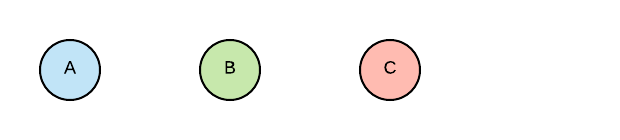
\includegraphics[width=8.5cm]{Images/Distribution1.png} }}%
%\qquad
%\qquad
%\subfloat[A new access point D is turned on between B and C. Now it has to pick a channel.]{{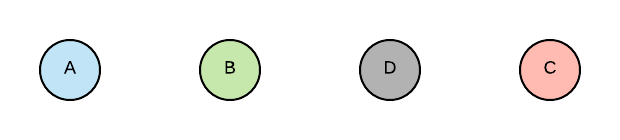
\includegraphics[width=8.5cm]{Images/Distribution2.png} }}%
%\qquad
%\qquad
%\subfloat[D has to pick the same channel as A, as it has the least  amount of interference]{{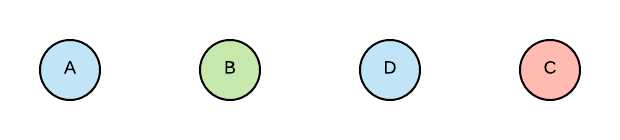
\includegraphics[width=8.5cm]{Images/Distribution3.png} }}%
%\qquad
%\qquad
%\subfloat[But this optimal distribution, where C gives its channel to D, can never be reached without coordination between access points.]{{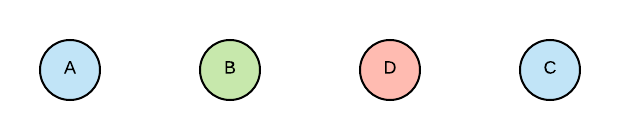
\includegraphics[width=8.5cm]{Images/Distribution4.png} }}%
%\caption{The channel distribution problem}%
%\label{fig:distribution}
%
%\squeezeup
%\end{figure}
%%This bring us to the punch line of the problem definition: finding a way to confine access points to high-impact groups. We have already established the motivation behind aiming for a decentralized solution - but to achieve this, access points have to find these groups on their own. It is easy to intuitively say that, for instance, an apartment building should be one group. It is less obvious to answer how all access points in an apartment building would identify the boundaries of the building and create a group on their own, entirely independent of an Internet service provider (and ideally also router brand). This boils down to a distributed clustering problem, where no access point has a global view of the landscape of neighbouring routers, and the cluster size
%can not surpass a given maximum size. This group creation method must be built relying solely on information that can be obtained from radio scans of the group's membering access points.

\section{Method}
To develop and test algorithms to form clusters in a way that creates groups of nodes that fulfill the requirements, we need to perform data gathering to have simulation
data. The report "Computing as a discipline" by the ACM Task Force \cite{Denning} introduces 3 paradigms for the computing discipline. Throughout this thesis we will follow the design paradigm from the report to build the programs required to address the problems presented in this thesis.

\section{Outline}
The structure of the thesis is as follows:

\begin{itemize}
	\item \textbf{Chapter 2: Background} \newline
	In the background chapter we look at the mechanisms of wireless technologies and the 802.11 standard. We look at why interference impacts 
		Wi-Fi so hard, and what countermeasures exists.

	\item \textbf{Chapter 3: Related Work} \newline
		Here we consider the work that has been done to minimize the impact of co-channel interference in different centralized solutions.
		We also look at technology that is aimed to work in a chaotic, distributed environment, that can possibly facilitate clustering in the real world.

	\item \textbf{Chapter 4: Data acquisition and data structure} \newline
		This chapter is dedicated to the creation of artificial network topologies that will be used to test algorithms under development.
		We present the data structure for how network topologies will be stored, and create a program that can visually represent the network topologies in a browser.

	\item \textbf{Chapter 5: Access point clustering}\newline
	Here the we phrase the requirements and specification of a distributed clustering algorithm fit to run on wireless access points.
	Then we use the data from chapter 4 to iteratively build and evaluate a clustering algorithm.

	\item \textbf{Chapter 6: Group communication and state synchronization} \newline
	This chapter is dedicated to looking at technologies and protocols that could facilitate a real world implementation of the algorithm suggested in chapter 5. 
	We also suggest an abstract architecture of how these components could coexist. 	

	\item \textbf{Chapter 7: Conclusion} \newline
	Finally we conclude by looking at what has been done, and consider if the problems in the problem statement have been addressed. Then we look at possible
		future work in this area, and what remains to do before the clustering algorithm can be implemented in the real world.  
\end{itemize}
%


